% Valentino Vranic
% Metody inzinierskej prace 2012/13

\documentclass{beamer}
\graphicspath{ {./assets/} }

%\usetheme{Warsaw}
%\usetheme{Antibes}
\usetheme{JuanLesPins}
%\usetheme{Goettingen}

\usecolortheme{seahorse}
%\usecolortheme{dolphin}
%\usecolortheme{rose}
% https://deic.uab.cat/~iblanes/beamer_gallery/
%\usecolortheme{beaver}

%\useoutertheme[]{sidebar}

\setbeamercovered{transparent}

\usepackage[slovak]{babel}
\usepackage[T1]{fontenc}
\usepackage[utf8]{inputenc}
\usepackage{url}

\usepackage{listings}

\lstset{language=C++,basicstyle=\fontsize{8}{9.6}\selectfont,showstringspaces=false,columns=fullflexible,identifierstyle=\ttfamily,keywordstyle=\bfseries,showstringspaces=false,columns=fullflexible}
%\lstset{language=C,basicstyle=\fontsize{10.5}{12.6}\selectfont,identifierstyle=\ttfamily,keywordstyle=\bfseries,showstringspaces=false,columns=fixed}

\def\BibTeX{\textsc{Bib}\kern-.08em\TeX} 

\newcommand{\footcite}[1]{\footnote{\tiny #1}}
\newcommand{\umlet}{.5}
\newcommand{\emp}[1]{\textit{\alert{#1}}}
\newcommand{\kw}[1]{\mbox{\textbf{#1}}}
\newcommand{\id}[1]{\texttt{#1}}
\newcommand{\stl}{\guillemotleft}
\newcommand{\str}{\guillemotright}

\newcommand{\lsti}{\lstinline[basicstyle=\fontsize{10.5}{12.1}\selectfont]}

\newcommand{\ssection}[1]{
	\section{#1}
	\begin{frame}[fragile=singleslide]\frametitle{}
	\Huge #1
	\end{frame}
}

\newcommand{\ssectionn}[1]{
	\section*{#1}
	\begin{frame}[fragile=singleslide]\frametitle{}
	\Huge #1
	\end{frame}
}

\newenvironment{program}{\begin{beamercolorbox}[rounded=true,shadow=true]{block body}\vspace{-4mm}}{\vspace{-2mm}\end{beamercolorbox}}

\setbeamercolor{fvystup}{fg=white,bg=black}
\newenvironment{vystup}{\begin{beamercolorbox}[rounded=true,shadow=true]{fvystup}}{\end{beamercolorbox}}

\newenvironment{poznamka}{\begin{beamercolorbox}[rounded=true,shadow=false]{block body}}{\end{beamercolorbox}}

\setbeamertemplate{footline}[page number]
{
%\insertpagenumber
%\begin{beamercolorbox}{section in head/foot}
%\vskip2pt\insertnavigation{\paperwidth}\vskip2pt
%\end{beamercolorbox}%
}



\author{Maksym Mertsalov}
%\url{www.fiit.stuba.sk/~vranic}, \url{vranic@fiit.stuba.sk}}
%{\tiny \url{www.fiit.stuba.sk/~vranic}, \url{vranic@fiit.stuba.sk}}
\institute{
	Ústav informatiky, informačných systémov a softvérového inžinierstva\\
	Fakulta informatiky a informačných technológií\\
	Slovenská technická univerzita v Bratislave}

\subtitle{\vspace{3mm} Metódy inžinierskej práce 2024/2025}

\title{Deep Learning vs. Machine Learning in digital marketing}

\date{\footnotesize 24. october 2024}


\begin{document}

\begin{frame}[fragile=singleslide]
\titlepage
\end{frame}


\begin{frame}[fragile=singleslide]\frametitle{O čom to je}
This article explores the best practices for developing an online advertising monitoring and promotion system powered by Artificial Intelligence (AI) and advanced algorithms. We’ll cover technologies like natural language processing (NLP) for content analysis, pattern recognition to detect trends, machine learning and deep learning for improved ad targeting and performance prediction, and data tracking for comprehensive monitoring.
This article is ideal for those aiming to optimize their advertising platforms. Whether you're seeking to improve ad accuracy, modernize data management, or stay competitive in the fast-evolving online advertising industry, you'll find valuable strategies here to elevate your ad systems\ldots
\end{frame}


\begin{frame}[fragile=singleslide]\frametitle{Prehľad}
\tableofcontents
\end{frame}


\section{Intro}
% príkaz \ssection by vytvoril zvláštný slajd s názvom časti - v krátkych prezentáciách to prekáža, lebo oberá o čas

\begin{frame}[fragile=singleslide]\frametitle{Intro}
Since the first brands emerged more than two centuries ago, advertising has undergone significant changes. Companies used to use newspapers, magazines, flyers, billboards and marketing calls to spread their messages. Later, they moved to mass media: television and radio.\par

However, digital technology is facilitating the emergence of a third sector: the online space. Search engines, websites and social media make advertising more ubiquitous than ever. \par
\end{frame}



\section{Image slide}

\begin{frame}[fragile=singleslide]\frametitle{Slide with first and second level bullet points}
\begin{itemize}
\item Nejaký text
\item Ďalší text -- \emph{zvýraznený text}
	\begin{itemize}
		\item This is second bullet point
		\begin{itemize}
			\item And third bullet point
		\end{itemize}
	\end{itemize}
\item \emp{Kľúčová poznámka} % príkaz definovaný v preambule

% odrážka s odkazom na zdroj:
\item Bol použitý balík beamer\footcite{\url{https://tug.ctan.org/macros/latex/contrib/beamer/doc/beameruserguide.pdf}}
\end{itemize}
\end{frame}


\begin{frame}[fragile=singleslide]\frametitle{Slajd len s obrázkom}
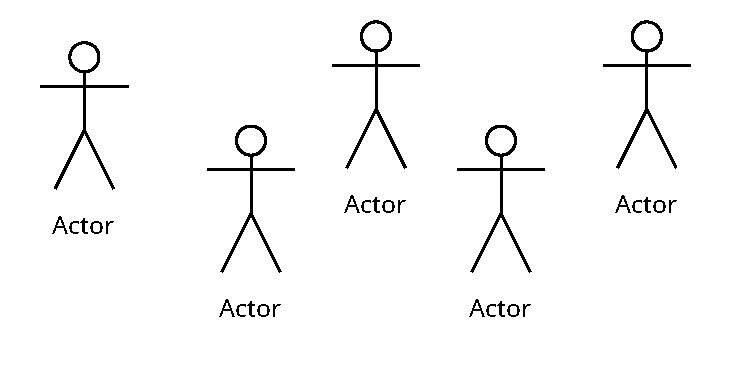
\includegraphics[scale=.35]{diagram_test1.pdf}
% pridajte vlastný obrázok a zrušte znák % pred príkazom \includegraphics vo formáte PDF prípadne PNG alebo JPG
% scale určuje veľkosť obrázku

{\tiny These are some people\ldots}
\end{frame}


\begin{frame}[fragile=singleslide]\frametitle{Zvýraznenie syntaxe}
\begin{itemize}
\item Na zvýraznenie syntaxe stačí použiť balík listings so správne nastaveným programovacím jazykom
\begin{lstlisting}
int na_druhu(int i) {
   return i * i;
}

int main() {
   printf("%d", na_druhu(118));
   return 0;
}
\end{lstlisting}

\item Jazyk C++ je ešte zaujímavejší: je multiparadigmový\footcite{\url{J. O. Coplien. Multi-Paradigm Design for C++. Addison-Wesley, 1998.}}
\end{itemize}
\end{frame}


\begin{frame}[fragile=singleslide]\frametitle{Rámiky}
\begin{poznamka}
Text možno uviesť v rámiku
\end{poznamka}

\begin{itemize}
\item Program

\begin{program}
\begin{lstlisting}
void main() {
   printf("%d", na_druhu(118));
}

void na_druhu(int i) {
   return i * i;
}
\end{lstlisting}
\end{program}

\item Výstup
\begin{vystup}
\begin{lstlisting}
13924
\end{lstlisting}
\end{vystup}

\end{itemize}
\end{frame}



\section*{Zhodnotenie a ďalšia práca}
% hviezdička zabezpečí, aby sa táto časť neocitla v prehľade prezentácie - každá prezentácia má zhodnotenie a prehľad by sa tým zbytočne zahlcoval

\begin{frame}[fragile=singleslide]\frametitle{Zhodnotenie a ďalšia práca}
\begin{itemize}
\item Každá prezentácia musí byť nejako uzavretá
\item Ale vždy je čo robiť ďalej\ldots{}
\end{itemize}
\end{frame}


\end{document}




Text \end{document} za príkazom \end{document} LaTeX ignoruje, takže tu môžete odkladať veci (aj celé slajdy), ktoré nechcete vymazať, lebo ich ešte možno budete potrebovať, avšak ich v danom momente nechcete mať v slajdoch.
